\newpage
\section*{Referencias}
\textbf{Básico: }
\begin{itemize}
	\item \textit{Problema 1.} Creado.
	\item \textit{Problema 2.} Creado. 
	\item \textit{Problema 3.} Creado.
	\item \textit{Problema 4.} Creado.
	\item \textit{Problema 5.} Problema 7, Nivel 1, 3a RONDA ZONAL de OMAPA, 2014.
\end{itemize}

\textbf{Avanzado: }
\begin{itemize}
	\item \textit{Problema 1.} Creado
	\item	\textit{Problema 2.} Problema 24, AMC8, 1997. 
	\item	\textit{Problema 3.} Problema 24, AMC10, 2008. 
	\item	\textit{Problema 4.} Problema 16.11 de Aops Algebra.
	\item	\textit{Problema 5.} Creado.
	\item \textit{Plus} 5.51 de Introduction to Geometry (AOPS).
\end{itemize}

%------------------------------------------------------------------------------------------------------------   
%----------------------------------                        BASICO                       ---------------------------------- 
%------------------------------------------------------------------------------------------------------------ 

\newpage
\section{Nivel Básico}\label{basico:2020_10_31}

\begin{center}
	\fbox{\fbox{\parbox{6in}{\centering
				\textbf{Tiempo mínimo: } 2 horas y 30 minutos.\\
				\textbf{Tiempo máximo: } 4 horas.\\	
				\textbf{Procedimientos: }Cada problema debe estar resuelto por escrito, en forma detallada, todos los pasos seguidos para su resolución deben estar bien explicados. Se le brindarán unas hojas grapadas, en la \textit{parte de enfrente} de cada hoja debe estar la solución de los problemas, la \textit{parte posterior} no se leerá pero las operaciones y cálculos deben hacerlos allí. \\
				\textbf{Puntaje: }Cada problema vale 50 puntos, son 5, para un total de 250 puntos.
				}}}
\end{center}

\begin{enumerate}
	\item \textbf{(50 puntos)}. Mario tiene una bóveda secreta en su habitación, para abrirla debe escribir tres números uno seguido de otro separados por un guión. Un día vió que su hermana estaba intentando adivinar la clave de su bóveda, entonces decidió cambiar su contraseña $12-5-13$ por una nueva. Al día siguiente de cambiar la contraseña intentó abrir la bóveda pero no logró acordarse de su nueva contraseña, solo recuerda que el producto de los números de ella es $210$. Cuántas son las posibles contraseñas que puede tener la bóveda de Mario? (Nota, el orden de introducir los números en la bóveda genera diferentes contraseñas, es decir, la contraseña $2-3-5$ es diferente de la $2-5-3$)
			
	\item \textbf{(50 puntos)}. Cuántos números naturales menores a 1000 dejan residuo 1 al ser divididos por 7? (Recuerde que residuo es el resto que queda al hacer una división, por ejemplo 23 deja residuo 2 al ser dividido por 7)
			
	
	\item \textbf{(50 puntos)}. En un colegio hay 170 estudiantes. Algunos de ellos asisten a la lúdica de Club matemático,  cine o fútbol, que se realizan por las tardes. Se sabe que
			\begin{itemize}
				\item 65 estudiantes asisten a Club matemático.
				\item 96 asisten a cine.
				\item 94 asisten a fútbol.
				\item 35 estudiantes asisten únicamente a la lúdica de cine.
				\item 42 asisten a cine y fútbol.
				\item 40 asisten a Club matemático y fútbol.
				\item 22 estudiantes asisten a las tres lúdicas.
			\end{itemize}
			Con base en la información anterior,
			\begin{enumerate}
				\item ¿Cuántos estudiantes están únicamente en el Club matemático?
				\item ¿Cuántos están únicamente en fútbol?
				\item ¿Cuántos de ellos asisten a cine o fútbol?
				\item ¿Cuántos asisten por lo menos a una de las lúdicas?
				\item ¿Cuántos estudiantes no asisten a ninguna lúdica?
			\end{enumerate}

				

	\item \textbf{(50 puntos)}. María está jugando con su calculadora, sin embargo su calculadora tiene dos problemas, el primero es que solo tiene un botón que lo que hace es multiplicar por 7 el número que esté en la pantalla y el otro problema es que en la pantalla solo muestra la cifra de las unidades del resultado. Por ejemplo, si había un 8 en la pantalla, al oprimir el botón quedará un 6, pues 6 es la cifra de las unidades de $8\times 7 =56$. Si al inicio María ve el número 7 en la pantalla, que número quedará en la pantalla luego de que María oprima el botón 2020 veces?
			
		
	\item \textbf{(50 puntos)}. Las cuadrículas del gráfico \ref{fig:omapa} son todas iguales. El área pintada de negro es de $72{\text{ cm}}^2$. Cuánto es la suma de las áreas de los triángulos $ABC$ y $CDE$?
	\begin{figure}[H]
		\centering
		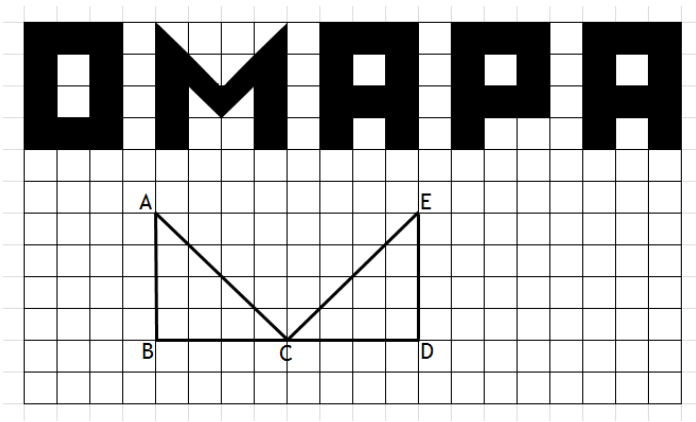
\includegraphics[width=0.7\linewidth]{2020_10_31/imgs/omapa}
		%\caption{}
		\label{fig:omapa}
	\end{figure}
	
\end{enumerate}



%------------------------------------------------------------------------------------------------------------   
%----------------------------------                        AVANZADO                       ---------------------------------- 
%------------------------------------------------------------------------------------------------------------ 

\newpage
\section{Nivel Avanzado}\label{avanzado:2020_10_31}

\begin{center}
	\fbox{\fbox{\parbox{6in}{\centering
				\textbf{Tiempo mínimo: } 2 horas y 30 minutos.\\
				\textbf{Tiempo máximo: } 4 horas.\\		
				\textbf{Procedimientos: }Cada problema debe estar resuelto por escrito, en forma detallada, todos los pasos seguidos para su resolución deben estar bien explicados. Se le brindarán unas hojas grapadas, en la \textit{parte de enfrente} de cada hoja debe estar la solución de los problemas, la \textit{parte posterior} no se leerá pero las operaciones y cálculos deben hacerlos allí. \\
				\textbf{Puntaje: }Cada problema vale 50 puntos, son 5, para un total de 250 puntos.
	}}}
\end{center}


\begin{enumerate}
	\item \textbf{(50 puntos)}. Cuántos números entre $-1000$ y $1000$ dejan residuo 5 al dividirlos por 9? (Recuerde que residuo es el resto que queda al hacer una división, por ejemplo -7 deja residuo 3 al ser dividido por 5, porque $-7=\color{red}5\color{black} \times (-2) + 3$. )
	

	\item \textbf{(50 puntos)}. En la figura \ref{fig:AV1} los vértices $A,C$ y $E$ están sobre el diámetro del circulo y el vértice $C$ divide al segmento $AE$ a razón de $2:3$. Los dos semicírculos, $ ABC $ y $ CDE $, dividen al circulo en una región superior (sombreada) y una región inferior. Cuál es la razón entre el área de la región superior y la de la región inferior.	
		\begin{figure}[H]
			\centering
			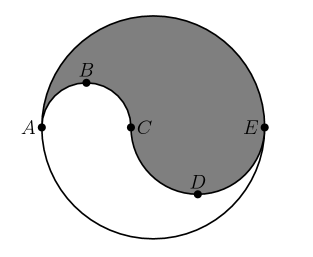
\includegraphics[width=0.5\linewidth]{2020_10_31/imgs/AV1}
			%\caption{}
			\label{fig:AV1}
		\end{figure}
	
	\item \textbf{(50 puntos)}.  Sea $ k = 2008 ^ 2 + 2 ^ {2008} $. ¿Cuál es el dígito de las unidades de $ k ^ 2 + 2 ^ k $?

	\item Sea $f(x)$ la función $f(x) = 3x+10$.
	\begin{enumerate}
		\item \textbf{(5 puntos)}. Calcular $f(2)$.		
		\item \textbf{(10 puntos)}. Calcular $f(f(3))$.
		\item \textbf{(35 puntos)}. Para que valores de $x$ se cumple que $f(f(x))=x?$
	\end{enumerate} 

	\item \textbf{(50 puntos)}. En total, en el club matemático de bachillerato hay 7 mujeres y 5 hombres. Necesito elegir un equipo con 5 personas para que participe de una prueba por equipos. De cuántas maneras diferentes puedo seleccionar el equipo
		\begin{enumerate}
			\item \textbf{(10 puntos)}. si no hay ninguna restricción para elegir los participantes del equipo? 
			\item \textbf{(15 puntos)}. si tienen que haber 2 mujeres y 3 hombres en el equipo? 
			\item \textbf{(25 puntos)}. si tienen que haber mas mujeres que hombres en el equipo? 
		\end{enumerate} 
	
	\item \textbf{PLUS (50 puntos)}. En la figura \ref{challege_551_aopgeo_ejer},  $\overline{BC} \parallel \overline{UR}$, $\overline{PS} \parallel \overline{BA}$ y $\overline{TQ} \parallel \overline{AC}$. Probar que
	\[
	\frac{PQ}{BC} + \frac{RS}{CA} + \frac{TU}{AB} = 1
	\]
	\begin{figure}[H]
		\centering
		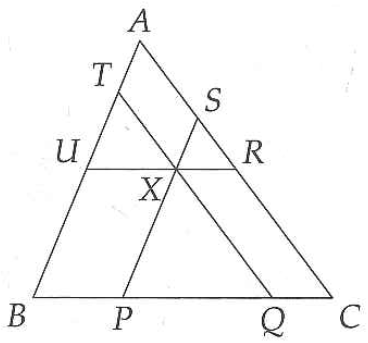
\includegraphics[width=0.5\linewidth]{2020_10_31/imgs/challege_551_aopgeo_ejer}		
	\end{figure}

\end{enumerate}